%%%%%%%%%%%%%%%%%%%%%%%%%%%%%%%%%%%%%%%%%%%%%%%%%%%%%%%%%%%%%%%%
%%                   Semester project 1	  	              %%
%%              Smart home energy monitoring   		      %%
%%                       Andrew Watson                        %%
%%                           MT-MA1                           %%
%%%%%%%%%%%%%%%%%%%%%%%%%%%%%%%%%%%%%%%%%%%%%%%%%%%%%%%%%%%%%%%%

%\documentclass[a4paper,draft]{article}
\documentclass[a4paper]{article}
% NB : enlever ``draft'' pour avoir les images!

\usepackage[english]{babel}
\usepackage[utf8]{inputenc}
\usepackage[T1]{fontenc} % for hyphenation of accentuated words
\usepackage{ae,aecompl}  % alternative to the fugly T1 fonts
\usepackage[pdftex]{graphicx} % modern graphics package
\usepackage{multirow}   % multiple rows in tables

%\usepackage{microtype}
%\usepackage{hyph-utf8}

\usepackage{wasysym}    % extended symbols
\usepackage{includes/mystyle}    % added styling
\usepackage{marvosym}   % euro symbol, among other things.
\usepackage[eurosym]{eurofont}

\usepackage[usenames,dvipsnames]{xcolor}  % if using PDFLaTeX
%\usepackage[usenames,dvips]{color}      % for regular LaTeX 

\usepackage{fancyhdr}   % fancy headers
\pagestyle{fancy}

%\usepackage{textcomp}  % some additionnal symbols
\usepackage{units}      % pretty units : \unit[val]{dim}
\usepackage{url}        % pretty urls
\usepackage{listings}   % pretty code listings \begin{lstlisting}
\usepackage{tikz} % pic/graph package. used for rounded corners :)

\graphicspath{{.}{./images/}}
\usepackage{subfigure} % multiple figures

%\addtocounter{secnumdepth}{1}  % number paragraphs

\usepackage{lscape}     % use landscape mode with \begin{landscape}
\usepackage{wrapfig}    % invoke Satan and wrap figures in text

\usepackage{hyperref}

\hypersetup{
    bookmarks=true,         % show bookmarks bar?
    unicode=true,          % non-Latin characters in Acrobat’s bookmarks
    pdftoolbar=true,        % show Acrobat’s toolbar?
    pdfmenubar=true,        % show Acrobat’s menu?
    pdffitwindow=true,     % window fit to page when opened
    pdfstartview={FitV},    % fits the width of the page to the window
    pdftitle={1st Semester Thesis},    % title
    pdfauthor={Andrew Watson},     % author
    pdfsubject={Wireless smart home network},   % subject of the document
    pdfcreator={Andrew Watson},   % creator of the document
    pdfproducer={EPFL}, % producer of the document
    pdfkeywords={AVR, embedded, ZigBee, Powerline, ELab}, % list of keywords
    pdfnewwindow=true,      % links in new window
    colorlinks=true,       % false: boxed links; true: colored links
    linkcolor=MidnightBlue,          % color of internal links
    citecolor=RoyalPurple,        % color of links to bibliography
    filecolor=magenta,      % color of file links
    urlcolor=DarkOrchid           % color of external links
}

\begin{document}
\begin{titlepage}
\nocite{*}      % to make sure bibliography appears in the correct order
  \begin{center}
     
     
    % Upper part of the page
    
\includegraphics[width=4cm]{logo_epfl}\\[1.5cm]
     
    \textsc{\LARGE Microengineering }\\[1.0cm]

    \textsc{\Large ELab - Semester Project}\\[0.1cm]

    \vfill 
     
    % Title
    \HRule \\[0.7cm]
    { \huge \bfseries Smart home wireless sensing}\\[0.4cm]

    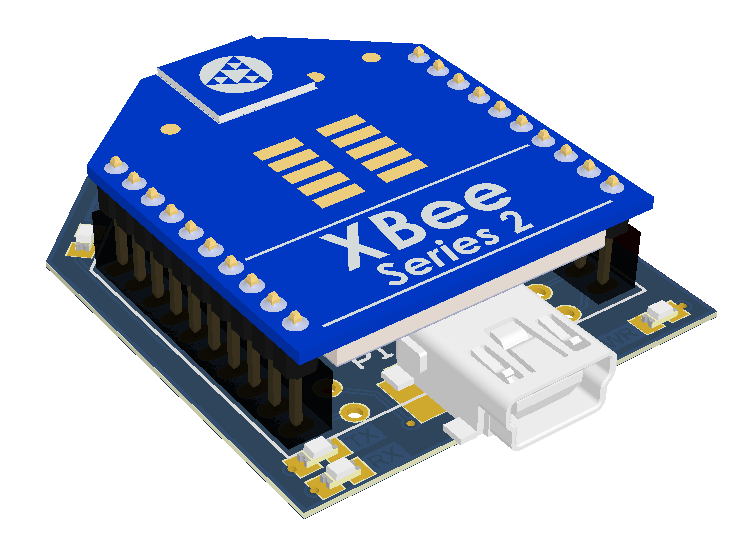
\includegraphics[width=0.6\textwidth]{title_pic} 
     
    \HRule \\[2.0cm]
     
    %% Author and supervisor
    \begin{minipage}{0.4\textwidth}
      \begin{flushleft} \large
        \emph{Author:} \\
        Andrew \textsc{Watson}\\[0.8cm]

        Microengineering\\
        Master - Semester 1\\[0.5cm]
      \end{flushleft}
    \end{minipage}
    \begin{minipage}{0.4\textwidth}
      \begin{flushright} \large
        \emph{Supervisor:} \\
        Maher \textsc{Kayal}\\[0.5cm]

        \emph{Assistants:} \\
        Fabrizio \textsc{Lo Conte}\\
        Laurent \textsc{Fabre}\\[0.5cm]
      \end{flushright}
    \end{minipage} \\[2cm]
     
    \vfill
     
    % Bottom of the page
    {\large \today}
     
  \end{center}

\end{titlepage}
%\maketitle

\newpage{}

%\fancyhead{}
\fancyfoot{}
\lhead{}
\cfoot{\thepage}        % numéro de page..
\lfoot{Semester Project}
%\rfoot{\today}
\rfoot{\today} %% TODO : fix the date

%\begin{abstract}
%\end{abstract}


%\renewcommand\contentsname{Plan}  % Rename ``Table des Matières''
\tableofcontents{}

\newpage

%%%% BEGIN : LSTLISTINGS CONFIG %%%%%%
%%%% TODO : MOVE TO SEPARATE FILE ONCE FINISHED %%%%%
%% see http://www.jorgemarsal.com/blog/2009/06/08/source-code-snippets-in-latex/
\lstset{language=C}
%\definecolor{lightgrey}{RGB}{200,200,200}
\definecolor{grey92}{gray}{0.92}
\definecolor{grey75}{gray}{0.75}
\definecolor{grey45}{gray}{0.45}


\lstdefinestyle{console}
{
  numbers=none,
  basicstyle=\bf\ttfamily,
  backgroundcolor=\color{grey92},
  frame=lrtb,
  framerule=0.5pt,
  linewidth=\textwidth,
}
\lstdefinestyle{avr-c}
{
  style=console
}

\lstset{
  style=console
}

%%%%%%% END : LSTLISTINGS CONFIG %%%%%%%%


\section*{Introduction}
\addcontentsline{toc}{section}{Introduction}
\markboth{Introduction}{\MakeUppercase{Introduction}}
This is the introduction for my semester project

\section{Context and previous work}
Here, I talk about Thierry's project, and a few words about the other projects,
and how they fit together as a system.

\section{Overview}
Describe how my system works, and why it's useful

\section{Recherche de solutions}
List some options that were considered and discarded, and why.

\subsection{Power supply}
Why NiMH? Why not LiPO? Why not use a DC-DC converter?

\subsection{Wireless}
Why ZigBee? Within ZigBee solutions, why XBees?

\subsection{Microcontroller}
Why go for an ATXMEGA?
Explain the reason for getting a 64-pin instead of the cheaper XMEGAxxA4.
Don't forget to mention : in the hardware design, only I/Os that are also
available on the 44 pin version were used. Also, because of the good modularity
of the XMEGA family, the code can be ported without any changes from one device
to another.

\section{Network topology}

Zigbee is designed to work well in a mesh configuration. However, this requires
some ``repeater'' nodes (routers) to be constantly on to relay transmissions
from the end nodes. Since the battery-powered devices cannot be expected to run
continuously, the network will function in a star topology.

In this configuration, the gateway device is powered from the grid, and the
wireless sensor nodes wake up at a given interval and transmit their data to the
gateway. The sensors manage their sleep themselves, and it is not necessary to
send them commands. This option has been disabled to save power, but it would be
possible to wake a module up periodically and listen for incoming transmissions.

In this setup, the router and coordinator automatically buffer packets until the
destination node wakes up.
\section{Hardware design}

Go over hardware in blocks

Explain the difference between receiver and emitters

Show details of sensor expansion port

\subsection{Base board}

Each sensor node consists of a basic board and a sensor add-on. The basic board
provides standard features common to all the nodes, such as network
connectivity, power management, and processing.

\subsubsection{Overview}

The main board is made up of several elements. At its core is an ATXMEGA. This
microcontroller was chosen mainly for its scalability and low power
requirements. The microcontroller communicates through a serial link with the
XBee, its radio transmitter.

The sensor nodes have a few on-board sensors which are available on all versions
of the board. These include an ambient light sensor, which is pointed towards
the front of the board, some measurements of supply voltages, as well as
temperature of the microcontroller. As the power usage is meant to be very low,
it was assumed that the temperature readings would not suffer very much from
the activity of the chip itself.

Power is supplied mainly by batteries which are placed directly on the board,
and can be recharged from an external interface. A power switch can be toggled
by the user to turn the node on and off.

\subsubsection{Microcontroller}

The current version of the board uses a 64-pin microcontroller, because it
was impossible to source a 44-pin version at design time. The schematics and
code were designed with a 44 pin microcontroller in mind, and it would be
trivial to adapt the design to the smaller version to reduce cost, and use less
space on the board.


\subsubsection{Power supply}
% TODO : insert picture of power supply design
The nodes can have various power sources. They were designed to function on two
AA batteries, which provide voltages between 2 and \unit{3.2}{V}. All components on
the board were chosen to operate in this voltage range.

To reduce the size requirements, the batteries are placed directly on the board,
on either side of the the radio transmitter.

On the left side of the board, a 4-pin JST header provides a connection to an
external charger (or solar power module). The power lines can be disconnected by
the main controller, and two communication lines are available for information
exchange between the sensor node and its power source. These lines are connected
to the ATXMEGA's USART lines in case serial communication is desired.

In addition to this, the input voltage can be measured with a voltage divider,
and disconnected if it is not needed. The ATXMEGA has a built-in module for
measuring its own supply voltage, using a 10x voltage divider with a 1\unit{V}
reference.

\subsubsection{Debug}

The nodes were designed to function the same way if the microcontroller was
replaced by a 44-pin version. This leaves one port unused on the ATMEGA64A3,
which was thus used as a debug port. Five pins are available on the right side
of the device to display status on an LED or to send debug data through USARTF0.

\subsubsection{Discarded features}

Several features originally included in the design or enumerated during the
design phase were discarded. I will go over some of these and explain the
reasons behind these choices.

\subsection{Sensor boards}

in its current state, the project has three sensor boards that can be installed
in the expansion port.

\subsubsection{Motion sensor}

% TODO : detect movement, low consumption but must be constantly powered (use
% analog comparator), needs min 5v

\subsubsection{Environmental sensors}

The environment sensing board is comprised of three sensors:

%\begin{enum}
%  \item Barometer
%  \item Temperature sensor
%  \item Capacitive humidity sensor
%\end{enum}


The barometer and temperature were both chosen for their low consumption and
easy communication (both use the I$^{2}$C bus on the expansion port).

The capacitive humidity sensor was chosen for it's price, but as a consequence,
it is very inaccurate and requires calibration.

\subsubsection{Light controller}

The final module is intended to control lights. It include connections for two
momentary switches, as well as two potentiometers which can be turned on and
off. With this module, the microcontroller can be configured to remain in deep
sleep and only awake on a hardware interruption generated by the switches, or to
wake up periodically to sample the potentiometer.

%%%%%%%%%%%%%%%%%%%%%%%%%%%%
% sampling the potentiometer

% extremities are connected between ground and a microcontroller pin. middle pin
% (find what that's called : cursor?) goes on adc input. pot can be turned on
% and off.



\section{Software considerations}

\section{Low-power design}

\section{Cost considerations}

For the sake of ease of development, some sacrifices were made in the area of
cost. For starters, the ATXMEGA is not very well suited to extremely low-cost
designs, as it is quite a lot more expensive than some competing solutions,
especially the PIC24F series and Cortex M3. On the other hand, it overs a very
modern architecture with many features to experiment with, which allows a lot of
freedom for development and experimenting.

% todo : mention choice of xmegaA3 over A4 and stuff
Moreover,

The other main area were cost was overlooked at the benefit of development time
is the wireless interface. Indeed, the average cost of an XBee module is
approximately \$22, whereas it is possible to source modules from Microchip for
instance that cost less than half as much. However, these require a one-time
purchase of an expensive software stack (which is not included), as well as a
more complex development. Therefore, the XBee modules were chosen, for their
seemingly ``plug-and-play'' functionality. If more time could be spend on the
development, it would be reasonable to expect to spend up to three times less on
the radio transmitter modules, while keeping the same functionality and
compatibility with the existing modules.

\section{Test results}

\section{Some examples of code}
\begin{lstlisting}[language=C]
  #define F_CPU 8000000UL
  #define Blah() do_nothing();

  #include <avr/io.h>
  #include "stuff.h"
  int main(void)
  {
    char blue = 0;
    int i = 0;

    for(i=0; i<10; i++)
    {
      // do stuff
      foo();
      bar();
    }
    code_example();
  }
\end{lstlisting}

There's also a way of including \code{code} inline.

\end{document}
